\documentclass[10pt]{beamer}

\usetheme[progressbar=frametitle]{metropolis}
\usepackage{appendixnumberbeamer}

\usepackage{booktabs}

\usepackage{pgfplots}
\usepgfplotslibrary{dateplot}

\usetikzlibrary{matrix}
\usetikzlibrary{arrows.meta}

\usepackage{xspace}

\title{An attack on Zarankiewicz's problem through SAT solving}
\author{Jeremy Tan}
\date{24 March 2022}
\institute{National University of Singapore}

\begin{document}
\maketitle

{\setbeamertemplate{frame footer}{\url{https://math.stackexchange.com/q/4335395}}
\begin{frame}{How I came to the problem}
  On 20 December 2021 I first saw a question on the Mathematics Stack Exchange (MSE) with an interesting premise:
  \begin{quote}
      How can 16 squares be shaded in a $7\times7$ grid so that for \textbf{any} choice of 3 rows and 3 columns, their 9 intersections \textbf{always} contain at least one shaded square (property A)?
  \end{quote}
  The actual question had lots of fluff and was eventually closed against my wishes. At this point I was unaware that this was a small case of Zarankiewicz's problem, but I had experience with Boolean satisfiability (SAT) solvers from my ATAP at DSO National Laboratories and saw an opportunity to apply them here.
\end{frame}
}

\begin{frame}{Solution}
  \begin{figure}
    \centering
    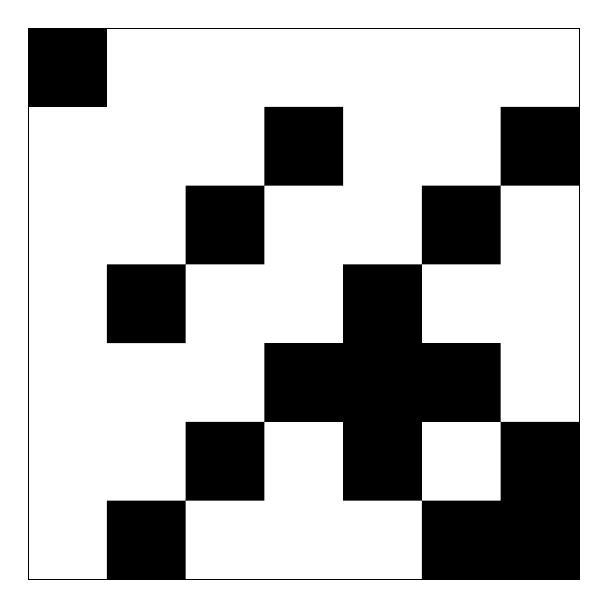
\begin{tikzpicture}\fill[black] (0,7) rectangle (1,6) (3,6) rectangle (4,5) (6,6) rectangle (7,5) (2,5) rectangle (3,4) (5,5) rectangle (6,4) (1,4) rectangle (2,3) (4,4) rectangle (5,3) (3,3) rectangle (4,2) (4,3) rectangle (5,2) (5,3) rectangle (6,2) (2,2) rectangle (3,1) (4,2) rectangle (5,1) (6,2) rectangle (7,1) (1,1) rectangle (2,0) (5,1) rectangle (6,0) (6,1) rectangle (7,0); \draw[black] (0,0) rectangle (7,7);\end{tikzpicture}
  \end{figure}
\end{frame}

\begin{frame}{Non-solution}
  \begin{figure}
    \centering
    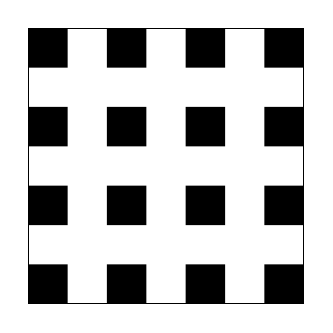
\begin{tikzpicture}[scale=0.5]\fill[black] (0,0) rectangle (1,1) (0,2) rectangle (1,3) (0,4) rectangle (1,5) (0,6) rectangle (1,7) (2,0) rectangle (3,1) (2,2) rectangle (3,3) (2,4) rectangle (3,5) (2,6) rectangle (3,7) (4,0) rectangle (5,1) (4,2) rectangle (5,3) (4,4) rectangle (5,5) (4,6) rectangle (5,7) (6,0) rectangle (7,1) (6,2) rectangle (7,3) (6,4) rectangle (7,5) (6,6) rectangle (7,7); \draw[black] (0,0) rectangle (7,7);\end{tikzpicture}
  \end{figure}
  \begin{itemize}
      \item Here the intersections of 1-indexed rows/columns 2, 4, 6 contain no shaded squares -- contiguity is not required.
      \item It is impossible to shade only 15 (and hence any fewer number of) squares in a $7\times7$ grid and satisfy property A. In fact the solution on the previous slide is unique up to problem symmetries (more on this later).
  \end{itemize}
\end{frame}

\begin{frame}{How I came to the problem}
  Using \href{https://github.com/arminbiere/cadical}{CaDiCaL}, the solver I used in my internship, and a (then rudimentary) Python script to generate the necessary files, I computed the fewest number of shaded squares needed to satisfy property A for grid sizes from $3\times3$ to $11\times11$:
  \begin{equation*}
      1,3,5,10,16,22,32,40,52,\mathbf{64}\dots
  \end{equation*}
  This sequence was not in the OEIS \textit{per se}, so I was encouraged to add it, but while my sequence was in the review queue Andrew Howroyd pointed out its inclusion as a column of an \href{https://oeis.org/A339635}{existing entry} -- I saw the link to Zarankiewicz's problem there and realised that the $11\times11$ term extended \href{https://oeis.org/A001198}{yet another sequence} for the first time in over 50 years.
\end{frame}

\begin{frame}{How I came to the problem}
  As soon as my sequence was accepted as \href{https://oeis.org/A350237}{A350237} I emailed my supervisors requesting a change of my FYP topic to Zarankiewicz's problem from a rather dry one involving algorithms for medians/centres under permutation distances. I am grateful to them as well as the FYP coordinators for allowing such a change.
\end{frame}

\begin{frame}{Definitions and scope}
  Zarankiewicz \cite{origin} defined his problem in the complementary manner to the MSE post:
  \begin{quote}
      What is the maximum number $z_{a,b}(m,n)$ of ones an $m\times n$ binary matrix can have if it is admissible, i.e.\ does not have an all-one $a\times b$ minor?
  \end{quote}
  As in Guy \cite{guy} I suppress indices whenever the matrix or minor is square; in fact my FYP only covers $2\times2$, $3\times3$ and $4\times4$ minors, so for example $\operatorname{A350237}(n)=n^2-z_3(n)$.
  
  Matrices attaining the maximum number of ones are termed \textit{maximal}. Beyond the values for $z$ I also computed all admissible \textit{square} maximal matrices \textit{up to permuting rows and columns and if applicable transposition}, since clearly an admissible matrix remains admissible under these symmetries.
\end{frame}

\begin{frame}{Arguments}
  Guy's 1969 paper \cite{guy} is still a very valuable reference for Zarankiewicz's problem, complete as it is with hand-computed tables of $z_{a,b}(m,n)$ for $2\le a,b\le4$ (no $a=b$ restriction) and a few extremely useful ``arguments''.
  \metroset{block=fill}
  \begin{block}{Argument A}
    An admissible matrix with column sums $c_i$ ($1\le i\le n$) satisfies $\sum_i\binom{c_i}a\le(b-1)\binom ma$, since otherwise the pigeonhole principle guarantees an all-one $a\times b$ minor.
  \end{block}
  \begin{block}{Argument I}
    Every minor of every admissible matrix is itself admissible.
  \end{block}
\end{frame}

\begin{frame}{Arguments}
    My SAT solving approach first assumes a value for $z_{a,b}(m,n)$; because of symmetries I only need to consider unordered partitions of the assumed number of ones across rows and across columns (row and column partitions). Arguments A and I usually eliminate a great many partitions from consideration, resulting in far less time needed to generate them through a simple lexicographic algorithm.
\end{frame}

\begin{frame}{Roman's bound}
  \metroset{block=fill}
  \begin{block}{Theorem \cite{roman}}
    For all integers $p\ge a-1$
		\begin{equation*}
			z_{a,b}(m,n)\le\left\lfloor\frac{b-1}{\binom p{a-1}}\binom ma+\frac{(p+1)(a-1)}an\right\rfloor
		\end{equation*}
		and equality holds with $p=a$ or $p=a-1$ when $\ell(m,a,b)\le n$, where $\ell(m,a,b)\approx\frac{b-1}{a+1}\binom ma$ is related to the hypergraph packing formulation of Zarankiewicz's problem.
  \end{block}
\end{frame}

\begin{frame}{Roman's bound}
  My tables for $z$ rely on the equality cases of this theorem -- and nothing else! Why?
  \begin{itemize}
      \item Guy's tables are known to contain errors (cf. \cite{heger}). One goal of this FYP is to independently verify those tables' entries as far as they extend, and then some.
      \item The structure of maximal matrices in this part of $(m,n)$-space can be summarised as ``column sums as equal as possible'' -- there are typically a huge number of solutions even after accounting for symmetries.
  \end{itemize}
\end{frame}

\begin{frame}{SAT formulation}
As explained in some other FYP presentations the norm for expressing SAT problems is the conjunctive normal form (CNF), a conjunction (AND) of clauses or disjunctions (ORs) of Boolean variables and their negations. For example
\begin{equation*}
    (\neg x_2\lor\neg x_3)\land(x_1\lor\neg x_2\lor x_3)\land(\neg x_1\lor x_3)
\end{equation*}
Formulating Zarankiewicz's problem for given parameters ($a,b,m,n$ and assumed $z_{a,b}(m,n)$) as a CNF instance is very simple -- the variables are the matrix entries and each minor engenders a clause stating that it has at least one zero entry:
\begin{equation*}
    \bigwedge_{(\text{all minors})}\bigvee_{(v\text{ in minor})}\neg v
\end{equation*}
\end{frame}

{\setbeamertemplate{frame footer}{*There may be none, which implies that the assumed $z$ value is too high without any need for SAT solving.}
\begin{frame}{SAT formulation}
With these clauses as a base I now follow Marijn Heule's cube-and-conquer paradigm \cite{cubeandconquer},
solving possibly several instances* for one parameter set where each instance enforces a row and column partition pair not ruled out by the arguments.
\begin{columns}[T,onlytextwidth]
    \column{0.5\textwidth}
      I force a row or column to have exactly its specified number of ones using the equality variation of Sinz's cardinality constraint encoding \cite{sinz} discussed in Wynn \cite{cardconstraint}, an encoding deemed in the latter reference as fastest and most efficient for general use.
    \column{0.5\textwidth}
      \begin{figure}
      \centering
      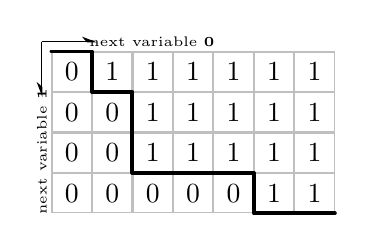
\begin{tikzpicture}
        \matrix(A)[matrix of nodes,minimum size=5mm,nodes={draw=lightgray},ampersand replacement=\&,matrix anchor=north west]{
        0\&1\&1\&1\&1\&1\&1\\
        0\&0\&1\&1\&1\&1\&1\\
        0\&0\&1\&1\&1\&1\&1\\
        0\&0\&0\&0\&0\&1\&1\\
        };
        \draw[line width=0.5mm,black,line join=round,line cap=round] (A-1-1.north west) -- (A-1-2.north west) -- (A-2-2.north west) -- (A-2-3.north west) -- (A-4-3.north west) -- (A-4-6.north west) -- (A-4-6.south west) -- (A-4-7.south east);
        \draw[arrows={-Stealth[harpoon]}] (0,0) -- (0.7,0);
        \draw[arrows={-Stealth[harpoon,swap]}] (0,0) -- (0,-0.7);
        \draw (1.4,0) node {\tiny{next variable \textbf{0}}};
        \draw (0,-1.4) node[rotate=90] {\tiny{next variable \textbf{1}}};
      \end{tikzpicture}
      \end{figure}
      \footnotesize{Sinz's encoding enforcing that exactly 4 of 11 variables are true.}
  \end{columns}
\end{frame}
}

\begin{frame}{SAT formulation}
To further break the symmetries of Zarankiewicz's problem -- reducing the total number of satisfying assignments for each instance while still allowing all non-isomorphic solutions -- within the SAT framework I require all columns and all rows with the same sum to be \textit{simultaneously} lexicographically sorted.
\begin{figure}
    \centering
    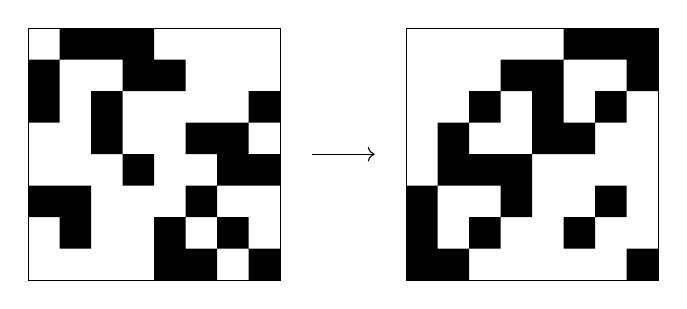
\begin{tikzpicture}
      \begin{scope}[scale=0.4,xshift=-10cm,yshift=-4cm]
            \fill[black] (0,2) rectangle (1,3) (0,5) rectangle (1,6) (0,6) rectangle (1,7) (1,1) rectangle (2,2) (1,2) rectangle (2,3) (1,7) rectangle (2,8) (2,4) rectangle (3,5) (2,5) rectangle (3,6) (2,7) rectangle (3,8) (3,3) rectangle (4,4) (3,6) rectangle (4,7) (3,7) rectangle (4,8) (4,0) rectangle (5,1) (4,1) rectangle (5,2) (4,6) rectangle (5,7) (5,0) rectangle (6,1) (5,2) rectangle (6,3) (5,4) rectangle (6,5) (6,1) rectangle (7,2) (6,3) rectangle (7,4) (6,4) rectangle (7,5) (7,0) rectangle (8,1) (7,3) rectangle (8,4) (7,5) rectangle (8,6);
            \draw (0,0) rectangle (8,8);
      \end{scope}
      \begin{scope}[scale=0.4,xshift=2cm,yshift=-4cm]
	        \fill[black] (0,3) rectangle (1,2) (0,2) rectangle (1,1) (0,1) rectangle (1,0) (1,5) rectangle (2,4) (1,4) rectangle (2,3) (1,1) rectangle (2,0) (2,6) rectangle (3,5) (2,4) rectangle (3,3) (2,2) rectangle (3,1) (3,7) rectangle (4,6) (3,4) rectangle (4,3) (3,3) rectangle (4,2) (4,7) rectangle (5,6) (4,6) rectangle (5,5) (4,5) rectangle (5,4) (5,8) rectangle (6,7) (5,5) rectangle (6,4) (5,2) rectangle (6,1) (6,8) rectangle (7,7) (6,6) rectangle (7,5) (6,3) rectangle (7,2) (7,8) rectangle (8,7) (7,7) rectangle (8,6) (7,1) rectangle (8,0);
			\draw (0,0) rectangle (8,8);
	    \end{scope}
	    \draw[->] (-0.4,0) -- (0.4,0);
    \end{tikzpicture}
\end{figure}
\end{frame}

\begin{frame}{SAT formulation}
\metroset{block=fill}
\begin{block}{Theorem}
  Every binary matrix $A$ can be made to satisfy the above property by alternately sorting same-sum rows and same-sum columns a finite number of times. In other words, no generality is lost here.
\end{block}
\begin{block}{Proof}
  The integral resource function $f(A)=\sum_{i=1}^m\sum_{j=1}^n2^{i+j-2}a_{ij}$ is clearly bounded and strictly increases or strictly decreases (depending on the sort order) every time two out-of-order rows or columns are swapped.
\end{block}
\end{frame}

\begin{frame}{Software used}
This lexicographic constraint eliminates most but not all isomorphic solutions; removing all isomorphs is equivalent to solving the graph isomorphism problem, which is better handled by a dedicated program such as Nauty's \texttt{shortg} \cite{nauty} than a SAT solver. Nevertheless, the constraint is very cheap to implement in CNF.

For the maximal square matrices, beyond finding all non-isomorphic solutions using \texttt{shortg} and noting their row and column partitions, I used GAP to compute their full automorphism groups with abstract descriptions. Finally, the SAT solver I used throughout my FYP proper was CaDiCaL's successor \href{https://github.com/arminbiere/kissat}{Kissat}.
\end{frame}

\begin{frame}{Results}
  \begin{table}
    \caption{$z_2(n)$ (OEIS \href{https://oeis.org/A072567}{A072567}). Italics denote new values; subscripts indicate the number of non-isomorphic solutions for that size if greater than 1.}
    \begin{tabular}{rcccccccc}
      \toprule
      $n$&1&2&3&4&5&6&7&8\\
      \midrule
      $z_2(n)$&1&3&6&9&12$_2$&16&21&24$_3$\\
      \bottomrule
      \toprule
      $n$&9&10&11&12&13&14&15&16\\
      \midrule
      $z_2(n)$&29&34&39&45&52&56&\textit{61}&\textit{67}$_4$\\
      \bottomrule
      \toprule
      $n$&17&18&19&20&21&22&23&24\\
      \midrule
      $z_2(n)$&\textit{74}&\textit{81}&\textit{88}&\textit{96}&\textit{105}&\textit{108}$_{10}$&\textit{115}&\textit{122}\\
      \bottomrule
    \end{tabular}
  \end{table}
\end{frame}

\begin{frame}{Results}
  \begin{table}
    \caption{$z_3(n)$ (OEIS \href{https://oeis.org/A350304}{A350304}).}
    \begin{tabular}{rcccccccc}
      \toprule
      $n$&1&2&3&4&5&6&7&8\\
      \midrule
      $z_3(n)$&1&4&8&13&20&26&33&42\\
      \bottomrule
      \toprule
      $n$&9&10&11&12&13&14&15&16\\
      \midrule
      $z_3(n)$&49$_7$&60&\textit{69}&\textit{80}$_2$&\textit{92}&\textit{105}&\textit{120}&\textit{128}\\
      \bottomrule
    \end{tabular}
  \end{table}
  \begin{table}
    \caption{$z_4(n)$.}
    \begin{tabular}{rcccccccccc}
      \toprule
      $n$&4&5&6&7&8&9&10&11&12&13\\
      \midrule
      $z_4(n)$&15&22&31&42&51&\textit{61}$_9$&\textit{74}&\textit{86}$_4$&\textit{100}$_2$&\textit{117}\\
      \bottomrule
    \end{tabular}
  \end{table}
\end{frame}

\begin{frame}{Results}
  Circulant maximal matrices feature most prominently in the $2\times2$ minor case, since it is easy to prove that $z_2(q^2+q+1)=(q+1)(q^2+q+1)$ where $q$ is a prime power using a projective plane construction \cite{reiman}, which itself can be rearranged into a circulant matrix \cite{singer}. But the motif also appears elsewhere:
  \begin{columns}[T,onlytextwidth]
    \column{0.25\textwidth}
      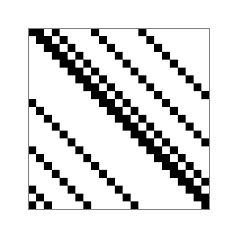
\begin{tikzpicture}\begin{scope}[scale=0.1]\fill[black] (0,23) rectangle (1,22) (1,23) rectangle (2,22) (3,23) rectangle (4,22) (8,23) rectangle (9,22) (14,23) rectangle (15,22) (1,22) rectangle (2,21) (2,22) rectangle (3,21) (4,22) rectangle (5,21) (9,22) rectangle (10,21) (15,22) rectangle (16,21) (2,21) rectangle (3,20) (3,21) rectangle (4,20) (5,21) rectangle (6,20) (10,21) rectangle (11,20) (16,21) rectangle (17,20) (3,20) rectangle (4,19) (4,20) rectangle (5,19) (6,20) rectangle (7,19) (11,20) rectangle (12,19) (17,20) rectangle (18,19) (4,19) rectangle (5,18) (5,19) rectangle (6,18) (7,19) rectangle (8,18) (12,19) rectangle (13,18) (18,19) rectangle (19,18) (5,18) rectangle (6,17) (6,18) rectangle (7,17) (8,18) rectangle (9,17) (13,18) rectangle (14,17) (19,18) rectangle (20,17) (6,17) rectangle (7,16) (7,17) rectangle (8,16) (9,17) rectangle (10,16) (14,17) rectangle (15,16) (20,17) rectangle (21,16) (7,16) rectangle (8,15) (8,16) rectangle (9,15) (10,16) rectangle (11,15) (15,16) rectangle (16,15) (21,16) rectangle (22,15) (8,15) rectangle (9,14) (9,15) rectangle (10,14) (11,15) rectangle (12,14) (16,15) rectangle (17,14) (22,15) rectangle (23,14) (0,14) rectangle (1,13) (9,14) rectangle (10,13) (10,14) rectangle (11,13) (12,14) rectangle (13,13) (17,14) rectangle (18,13) (1,13) rectangle (2,12) (10,13) rectangle (11,12) (11,13) rectangle (12,12) (13,13) rectangle (14,12) (18,13) rectangle (19,12) (2,12) rectangle (3,11) (11,12) rectangle (12,11) (12,12) rectangle (13,11) (14,12) rectangle (15,11) (19,12) rectangle (20,11) (3,11) rectangle (4,10) (12,11) rectangle (13,10) (13,11) rectangle (14,10) (15,11) rectangle (16,10) (20,11) rectangle (21,10) (4,10) rectangle (5,9) (13,10) rectangle (14,9) (14,10) rectangle (15,9) (16,10) rectangle (17,9) (21,10) rectangle (22,9) (5,9) rectangle (6,8) (14,9) rectangle (15,8) (15,9) rectangle (16,8) (17,9) rectangle (18,8) (22,9) rectangle (23,8) (0,8) rectangle (1,7) (6,8) rectangle (7,7) (15,8) rectangle (16,7) (16,8) rectangle (17,7) (18,8) rectangle (19,7) (1,7) rectangle (2,6) (7,7) rectangle (8,6) (16,7) rectangle (17,6) (17,7) rectangle (18,6) (19,7) rectangle (20,6) (2,6) rectangle (3,5) (8,6) rectangle (9,5) (17,6) rectangle (18,5) (18,6) rectangle (19,5) (20,6) rectangle (21,5) (3,5) rectangle (4,4) (9,5) rectangle (10,4) (18,5) rectangle (19,4) (19,5) rectangle (20,4) (21,5) rectangle (22,4) (4,4) rectangle (5,3) (10,4) rectangle (11,3) (19,4) rectangle (20,3) (20,4) rectangle (21,3) (22,4) rectangle (23,3) (0,3) rectangle (1,2) (5,3) rectangle (6,2) (11,3) rectangle (12,2) (20,3) rectangle (21,2) (21,3) rectangle (22,2) (1,2) rectangle (2,1) (6,2) rectangle (7,1) (12,2) rectangle (13,1) (21,2) rectangle (22,1) (22,2) rectangle (23,1) (0,1) rectangle (1,0) (2,1) rectangle (3,0) (7,1) rectangle (8,0) (13,1) rectangle (14,0) (22,1) rectangle (23,0); \draw[black!50] (0,0) rectangle (23,23);\end{scope}\end{tikzpicture}
      $z_2(23)$
    \column{0.25\textwidth}
      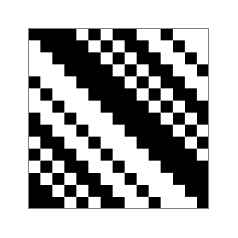
\begin{tikzpicture}\begin{scope}[scale=0.153]\fill[black] (0,0) rectangle (15,15); \fill[white] (4,15) rectangle (5,14) (6,15) rectangle (7,14) (9,15) rectangle (10,14) (10,15) rectangle (11,14) (12,15) rectangle (13,14) (13,15) rectangle (14,14) (14,15) rectangle (15,14) (0,14) rectangle (1,13) (5,14) rectangle (6,13) (7,14) rectangle (8,13) (10,14) rectangle (11,13) (11,14) rectangle (12,13) (13,14) rectangle (14,13) (14,14) rectangle (15,13) (0,13) rectangle (1,12) (1,13) rectangle (2,12) (6,13) rectangle (7,12) (8,13) rectangle (9,12) (11,13) rectangle (12,12) (12,13) rectangle (13,12) (14,13) rectangle (15,12) (0,12) rectangle (1,11) (1,12) rectangle (2,11) (2,12) rectangle (3,11) (7,12) rectangle (8,11) (9,12) rectangle (10,11) (12,12) rectangle (13,11) (13,12) rectangle (14,11) (1,11) rectangle (2,10) (2,11) rectangle (3,10) (3,11) rectangle (4,10) (8,11) rectangle (9,10) (10,11) rectangle (11,10) (13,11) rectangle (14,10) (14,11) rectangle (15,10) (0,10) rectangle (1,9) (2,10) rectangle (3,9) (3,10) rectangle (4,9) (4,10) rectangle (5,9) (9,10) rectangle (10,9) (11,10) rectangle (12,9) (14,10) rectangle (15,9) (0,9) rectangle (1,8) (1,9) rectangle (2,8) (3,9) rectangle (4,8) (4,9) rectangle (5,8) (5,9) rectangle (6,8) (10,9) rectangle (11,8) (12,9) rectangle (13,8) (1,8) rectangle (2,7) (2,8) rectangle (3,7) (4,8) rectangle (5,7) (5,8) rectangle (6,7) (6,8) rectangle (7,7) (11,8) rectangle (12,7) (13,8) rectangle (14,7) (2,7) rectangle (3,6) (3,7) rectangle (4,6) (5,7) rectangle (6,6) (6,7) rectangle (7,6) (7,7) rectangle (8,6) (12,7) rectangle (13,6) (14,7) rectangle (15,6) (0,6) rectangle (1,5) (3,6) rectangle (4,5) (4,6) rectangle (5,5) (6,6) rectangle (7,5) (7,6) rectangle (8,5) (8,6) rectangle (9,5) (13,6) rectangle (14,5) (1,5) rectangle (2,4) (4,5) rectangle (5,4) (5,5) rectangle (6,4) (7,5) rectangle (8,4) (8,5) rectangle (9,4) (9,5) rectangle (10,4) (14,5) rectangle (15,4) (0,4) rectangle (1,3) (2,4) rectangle (3,3) (5,4) rectangle (6,3) (6,4) rectangle (7,3) (8,4) rectangle (9,3) (9,4) rectangle (10,3) (10,4) rectangle (11,3) (1,3) rectangle (2,2) (3,3) rectangle (4,2) (6,3) rectangle (7,2) (7,3) rectangle (8,2) (9,3) rectangle (10,2) (10,3) rectangle (11,2) (11,3) rectangle (12,2) (2,2) rectangle (3,1) (4,2) rectangle (5,1) (7,2) rectangle (8,1) (8,2) rectangle (9,1) (10,2) rectangle (11,1) (11,2) rectangle (12,1) (12,2) rectangle (13,1) (3,1) rectangle (4,0) (5,1) rectangle (6,0) (8,1) rectangle (9,0) (9,1) rectangle (10,0) (11,1) rectangle (12,0) (12,1) rectangle (13,0) (13,1) rectangle (14,0); \draw[black!50] (0,0) rectangle (15,15);\end{scope}\end{tikzpicture}
      $z_3(15)$
    \column{0.25\textwidth}
      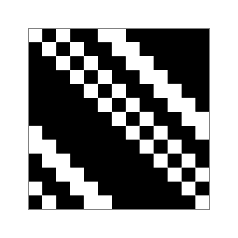
\begin{tikzpicture}\begin{scope}[scale=0.177]\fill[black] (0,0) rectangle (13,13); \fill[white] (0,13) rectangle (1,12) (2,13) rectangle (3,12) (5,13) rectangle (6,12) (6,13) rectangle (7,12) (1,12) rectangle (2,11) (3,12) rectangle (4,11) (6,12) rectangle (7,11) (7,12) rectangle (8,11) (2,11) rectangle (3,10) (4,11) rectangle (5,10) (7,11) rectangle (8,10) (8,11) rectangle (9,10) (3,10) rectangle (4,9) (5,10) rectangle (6,9) (8,10) rectangle (9,9) (9,10) rectangle (10,9) (4,9) rectangle (5,8) (6,9) rectangle (7,8) (9,9) rectangle (10,8) (10,9) rectangle (11,8) (5,8) rectangle (6,7) (7,8) rectangle (8,7) (10,8) rectangle (11,7) (11,8) rectangle (12,7) (6,7) rectangle (7,6) (8,7) rectangle (9,6) (11,7) rectangle (12,6) (12,7) rectangle (13,6) (0,6) rectangle (1,5) (7,6) rectangle (8,5) (9,6) rectangle (10,5) (12,6) rectangle (13,5) (0,5) rectangle (1,4) (1,5) rectangle (2,4) (8,5) rectangle (9,4) (10,5) rectangle (11,4) (1,4) rectangle (2,3) (2,4) rectangle (3,3) (9,4) rectangle (10,3) (11,4) rectangle (12,3) (2,3) rectangle (3,2) (3,3) rectangle (4,2) (10,3) rectangle (11,2) (12,3) rectangle (13,2) (0,2) rectangle (1,1) (3,2) rectangle (4,1) (4,2) rectangle (5,1) (11,2) rectangle (12,1) (1,1) rectangle (2,0) (4,1) rectangle (5,0) (5,1) rectangle (6,0) (12,1) rectangle (13,0); \draw[black!50] (0,0) rectangle (13,13);\end{scope}\end{tikzpicture}
      $z_4(13)$
    \column{0.25\textwidth}
      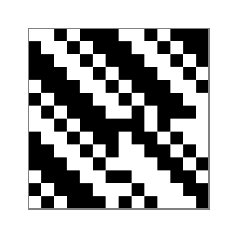
\begin{tikzpicture}\begin{scope}[scale=0.164]\fill[black] (0,0) rectangle (14,14); \fill[white] (0,14) rectangle (1,13) (1,14) rectangle (2,13) (3,14) rectangle (4,13) (7,14) rectangle (8,13) (8,14) rectangle (9,13) (10,14) rectangle (11,13) (1,13) rectangle (2,12) (2,13) rectangle (3,12) (4,13) rectangle (5,12) (8,13) rectangle (9,12) (9,13) rectangle (10,12) (11,13) rectangle (12,12) (2,12) rectangle (3,11) (3,12) rectangle (4,11) (5,12) rectangle (6,11) (9,12) rectangle (10,11) (10,12) rectangle (11,11) (12,12) rectangle (13,11) (3,11) rectangle (4,10) (4,11) rectangle (5,10) (6,11) rectangle (7,10) (10,11) rectangle (11,10) (11,11) rectangle (12,10) (13,11) rectangle (14,10) (0,10) rectangle (1,9) (4,10) rectangle (5,9) (5,10) rectangle (6,9) (7,10) rectangle (8,9) (11,10) rectangle (12,9) (12,10) rectangle (13,9) (1,9) rectangle (2,8) (5,9) rectangle (6,8) (6,9) rectangle (7,8) (8,9) rectangle (9,8) (12,9) rectangle (13,8) (13,9) rectangle (14,8) (0,8) rectangle (1,7) (2,8) rectangle (3,7) (6,8) rectangle (7,7) (7,8) rectangle (8,7) (9,8) rectangle (10,7) (13,8) rectangle (14,7) (0,7) rectangle (1,6) (1,7) rectangle (2,6) (3,7) rectangle (4,6) (9,7) rectangle (10,6) (11,7) rectangle (12,6) (12,7) rectangle (13,6) (13,7) rectangle (14,6) (1,6) rectangle (2,5) (2,6) rectangle (3,5) (4,6) rectangle (5,5) (7,6) rectangle (8,5) (10,6) rectangle (11,5) (12,6) rectangle (13,5) (13,6) rectangle (14,5) (2,5) rectangle (3,4) (3,5) rectangle (4,4) (5,5) rectangle (6,4) (7,5) rectangle (8,4) (8,5) rectangle (9,4) (11,5) rectangle (12,4) (13,5) rectangle (14,4) (3,4) rectangle (4,3) (4,4) rectangle (5,3) (6,4) rectangle (7,3) (7,4) rectangle (8,3) (8,4) rectangle (9,3) (9,4) rectangle (10,3) (12,4) rectangle (13,3) (0,3) rectangle (1,2) (4,3) rectangle (5,2) (5,3) rectangle (6,2) (8,3) rectangle (9,2) (9,3) rectangle (10,2) (10,3) rectangle (11,2) (13,3) rectangle (14,2) (1,2) rectangle (2,1) (5,2) rectangle (6,1) (6,2) rectangle (7,1) (7,2) rectangle (8,1) (9,2) rectangle (10,1) (10,2) rectangle (11,1) (11,2) rectangle (12,1) (0,1) rectangle (1,0) (2,1) rectangle (3,0) (6,1) rectangle (7,0) (8,1) rectangle (9,0) (10,1) rectangle (11,0) (11,1) rectangle (12,0) (12,1) rectangle (13,0); \draw[black!50] (0,0) rectangle (14,14);\end{scope}\end{tikzpicture}
      $z_3(14)$
  \end{columns}
\end{frame}

\begin{frame}{Results}
    Proving uniqueness of the maximal matrix for $z_2(23)$ required more than just SAT solving; a count using Marc Thurley's \href{https://github.com/marcthurley/sharpSAT}{sharpSAT} revealed exactly $6^6=46656$ instance solutions even after imposing the cardinality and lexicographic constraints. For this case I therefore took one maximal matrix and successfully generated $6^6$ distinct instance solutions by randomly permuting, then alternately sorting its rows and columns (the arguments had already ruled out all row and column partitions except the most level one, $(5^{23})\ (5^{23})$), thereby showing that all instance solutions were isomorphic to one another.
\end{frame}

\begin{frame}{Results}
    \begin{columns}[T,onlytextwidth]
    \column{0.45\textwidth}
      Maximal matrices for $z_a(m)$ where $m\le2a$ are simply described and unique by a paper of Yang \cite{yang}, but they get extremely complicated as soon as $m>2a$. \textit{Every} such matrix found, however, is not totally asymmetric, even those without a transpose symmetry (example on right), suggesting that a purely random search like that done in \cite{collins} is unlikely to yield maximal matrices.
    \column{0.5\textwidth}
      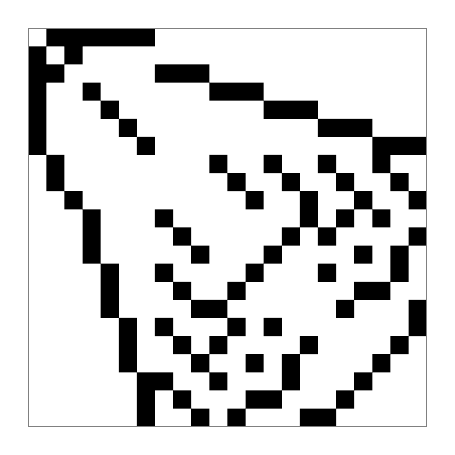
\begin{tikzpicture}\begin{scope}[scale=0.23]\fill[black] (1,22) rectangle (2,21) (2,22) rectangle (3,21) (3,22) rectangle (4,21) (4,22) rectangle (5,21) (5,22) rectangle (6,21) (6,22) rectangle (7,21) (0,21) rectangle (1,20) (2,21) rectangle (3,20) (0,20) rectangle (1,19) (1,20) rectangle (2,19) (7,20) rectangle (8,19) (8,20) rectangle (9,19) (9,20) rectangle (10,19) (0,19) rectangle (1,18) (3,19) rectangle (4,18) (10,19) rectangle (11,18) (11,19) rectangle (12,18) (12,19) rectangle (13,18) (0,18) rectangle (1,17) (4,18) rectangle (5,17) (13,18) rectangle (14,17) (14,18) rectangle (15,17) (15,18) rectangle (16,17) (0,17) rectangle (1,16) (5,17) rectangle (6,16) (16,17) rectangle (17,16) (17,17) rectangle (18,16) (18,17) rectangle (19,16) (0,16) rectangle (1,15) (6,16) rectangle (7,15) (19,16) rectangle (20,15) (20,16) rectangle (21,15) (21,16) rectangle (22,15) (1,15) rectangle (2,14) (10,15) rectangle (11,14) (13,15) rectangle (14,14) (16,15) rectangle (17,14) (19,15) rectangle (20,14) (1,14) rectangle (2,13) (11,14) rectangle (12,13) (14,14) rectangle (15,13) (17,14) rectangle (18,13) (20,14) rectangle (21,13) (2,13) rectangle (3,12) (12,13) rectangle (13,12) (15,13) rectangle (16,12) (18,13) rectangle (19,12) (21,13) rectangle (22,12) (3,12) rectangle (4,11) (7,12) rectangle (8,11) (15,12) rectangle (16,11) (17,12) rectangle (18,11) (19,12) rectangle (20,11) (3,11) rectangle (4,10) (8,11) rectangle (9,10) (14,11) rectangle (15,10) (16,11) rectangle (17,10) (21,11) rectangle (22,10) (3,10) rectangle (4,9) (9,10) rectangle (10,9) (13,10) rectangle (14,9) (18,10) rectangle (19,9) (20,10) rectangle (21,9) (4,9) rectangle (5,8) (7,9) rectangle (8,8) (12,9) rectangle (13,8) (16,9) rectangle (17,8) (20,9) rectangle (21,8) (4,8) rectangle (5,7) (8,8) rectangle (9,7) (11,8) rectangle (12,7) (18,8) rectangle (19,7) (19,8) rectangle (20,7) (4,7) rectangle (5,6) (9,7) rectangle (10,6) (10,7) rectangle (11,6) (17,7) rectangle (18,6) (21,7) rectangle (22,6) (5,6) rectangle (6,5) (7,6) rectangle (8,5) (11,6) rectangle (12,5) (13,6) rectangle (14,5) (21,6) rectangle (22,5) (5,5) rectangle (6,4) (8,5) rectangle (9,4) (10,5) rectangle (11,4) (15,5) rectangle (16,4) (20,5) rectangle (21,4) (5,4) rectangle (6,3) (9,4) rectangle (10,3) (12,4) rectangle (13,3) (14,4) rectangle (15,3) (19,4) rectangle (20,3) (6,3) rectangle (7,2) (7,3) rectangle (8,2) (10,3) rectangle (11,2) (14,3) rectangle (15,2) (18,3) rectangle (19,2) (6,2) rectangle (7,1) (8,2) rectangle (9,1) (12,2) rectangle (13,1) (13,2) rectangle (14,1) (17,2) rectangle (18,1) (6,1) rectangle (7,0) (9,1) rectangle (10,0) (11,1) rectangle (12,0) (15,1) rectangle (16,0) (16,1) rectangle (17,0); \draw[black!50] (0,0) rectangle (22,22);\end{scope}\end{tikzpicture}
      $z_2(22)$ -- has $S_4$ of order 24 as its automorphism group
    \end{columns}
\end{frame}

\begin{frame}{Limitations and future work}
    I did all of the SAT solving on a single laptop computer (my own) using Kissat, which is a single-processor solver. There was thus a ``natural'' limit of $z\approx100$ to the range of the table I could complete within reasonable time. My ideas for future work include:
    \begin{itemize}
        \item Taking cube-and-conquer to its fullest potential for Zarankiewicz's problem by further splitting into instances with \textit{partially assigned matrices} and distributing the larger number of instances across many processors (e.g. Charity Engine).
        \item Exploring other ways to obtain upper and lower bounds on the $z$-function, such as the ``neighbouring theorem'' of Collins \cite{collins}.
        \item Applying SAT solving to cases with non-square minors -- no part of my approach requires square minors.
    \end{itemize}
\end{frame}

\begin{frame}{Links}
  My full thesis, with tables for $z_{\{2,3,4\}}(m,n)$ and a complete listing of maximal square matrices, has been published on the arXiv at
  \begin{center}
    \url{https://arxiv.org/abs/2203.02283}
  \end{center}
  Supporting code can be found at
  \begin{center}
    \url{https://github.com/Parcly-Taxel/Kyoto}
  \end{center}
\end{frame}

{\setbeamercolor{palette primary}{fg=black,bg=yellow}
\begin{frame}[standout]
  Questions?
\end{frame}
}

\appendix
\begin{frame}[allowframebreaks]{References}
  \bibliography{refs}
  \bibliographystyle{abbrv}
\end{frame}
\end{document}
